\documentclass[12pt, a4paper]{article}
\usepackage[margin = 1in, top=1.3in, bottom = 0.9in]{geometry}
\usepackage[english]{babel}
\usepackage[utf8]{inputenc}
\usepackage{fancyhdr}
\usepackage{amsmath}
\usepackage{bm}
\usepackage{graphicx}
\usepackage{subcaption}
\usepackage{float}
\usepackage[font=small,labelfont=bf]{caption}
 
\pagestyle{fancy}
\fancyhf{}
\rhead{\small{Shaan Ul Haque(180070053)\\ Samarth Singh (180050090) \\ Niraj Mahajan (180050069)}}
\lhead{CS-663 Assignment-5 : Question 4}
\rfoot{Page 1.\thepage}
 
\begin{document}
\vspace*{-22pt}
\section{Ideal LPF on the image}
Original Image and its Fourier Transform are shown in fig. below.\\
\begin{figure}[H]
  \centering
  \begin{subfigure}[b]{0.37\linewidth}
    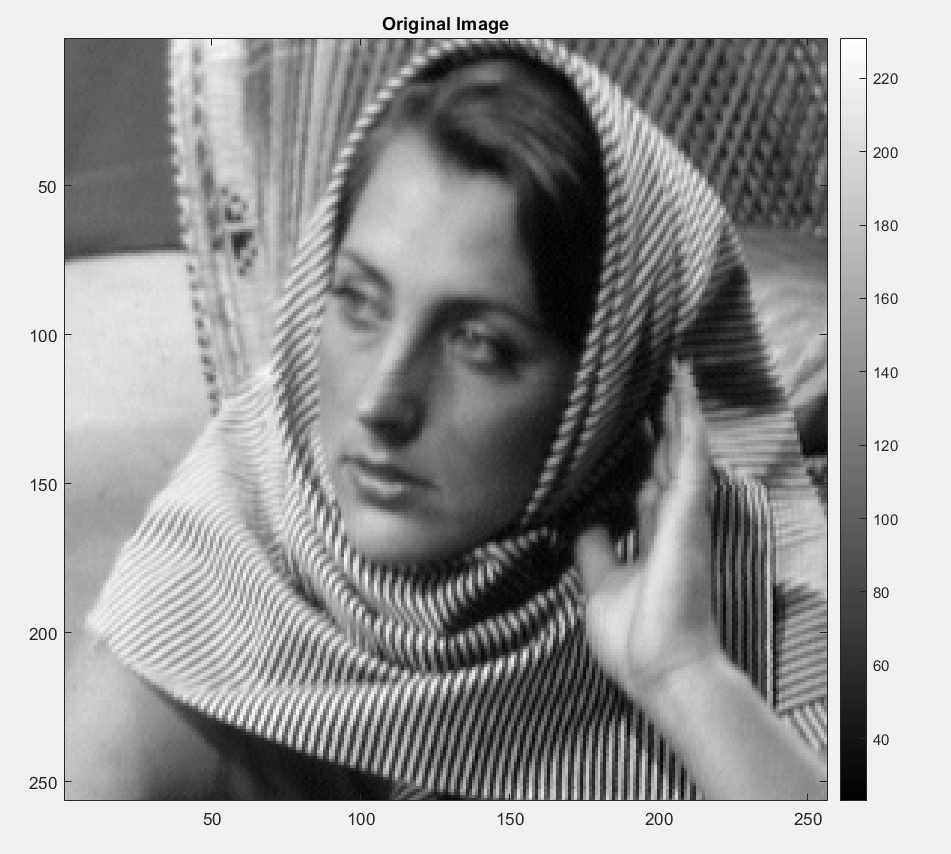
\includegraphics[width=\linewidth]{Screenshot (263).png}
    \caption{Original Image}
  \end{subfigure}
  \begin{subfigure}[b]{0.37\linewidth}
    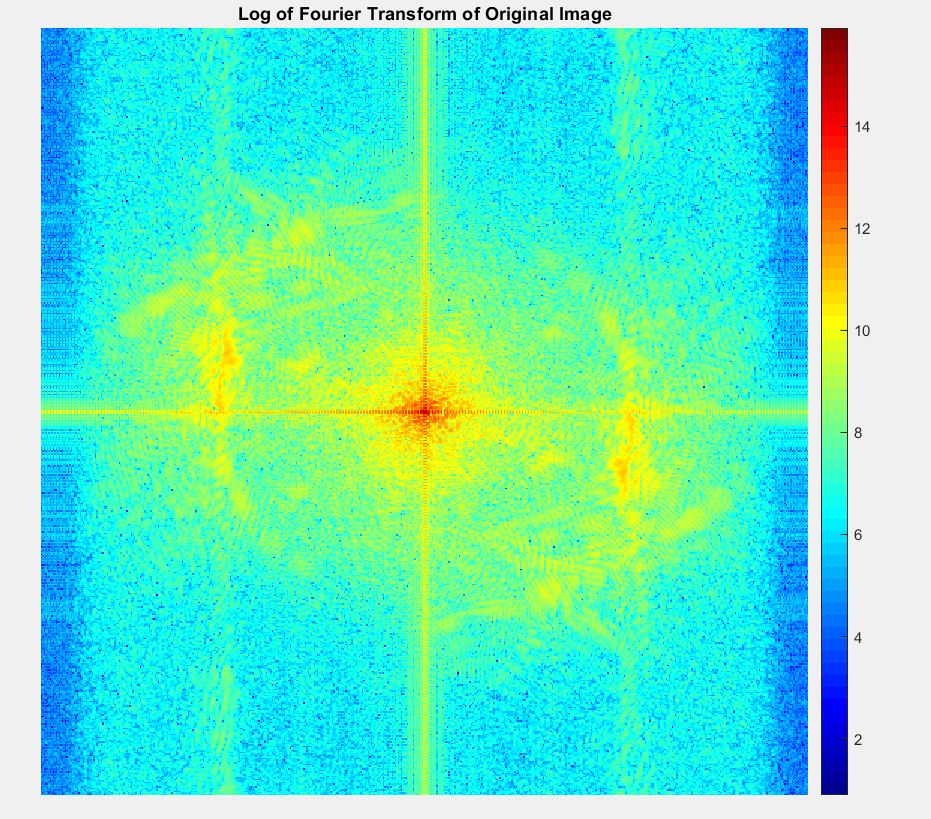
\includegraphics[width=\linewidth]{Screenshot (264).png}
    \caption{Fourier Transform}
  \end{subfigure}
  \caption{}
  \label{fig:1}
\end{figure}

We want to pass this image through an ideal lpf and see its effect on the image. Ideal low pass filter is defined by the following equation:
\begin{equation*}
    H(u, v) = 1  \ ;\  if \ u^2 + v^2 <= D^2
\end{equation*}
\begin{equation*}
     H(u, v) = 0  ; otherwise
\end{equation*}
\subsection{Cutoff frequency $|D|=40$}
The frequency response corresponding the filter is shown below.
\begin{figure}[h!]
  \centering
    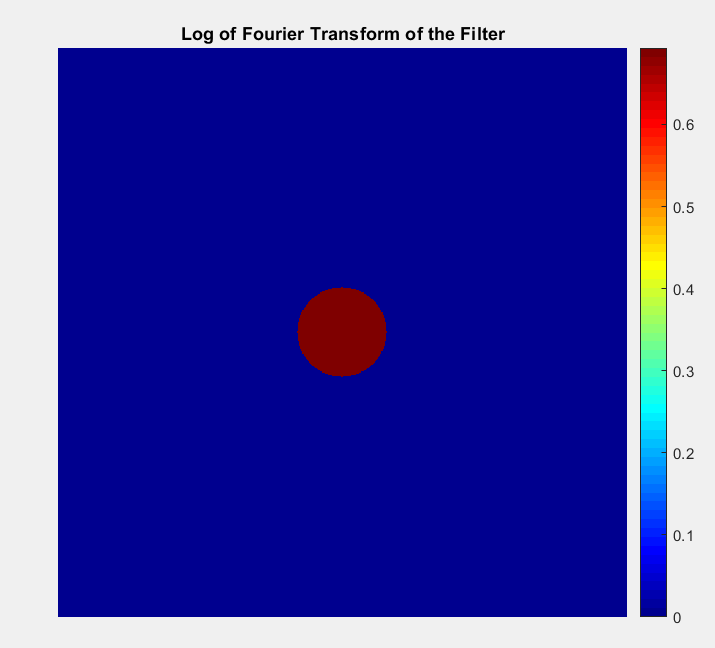
\includegraphics[scale=0.4]{Screenshot (276).png}
    \caption{Frequency response of an ideal LPF with cutoff frequency $|\omega|=40$}
  \label{fig:2}
\end{figure}

\clearpage

Image and the corresponding Fourier Transform are shown in fig. given below.
\begin{figure}[H]
  \centering
  \begin{subfigure}[b]{0.37\linewidth}
    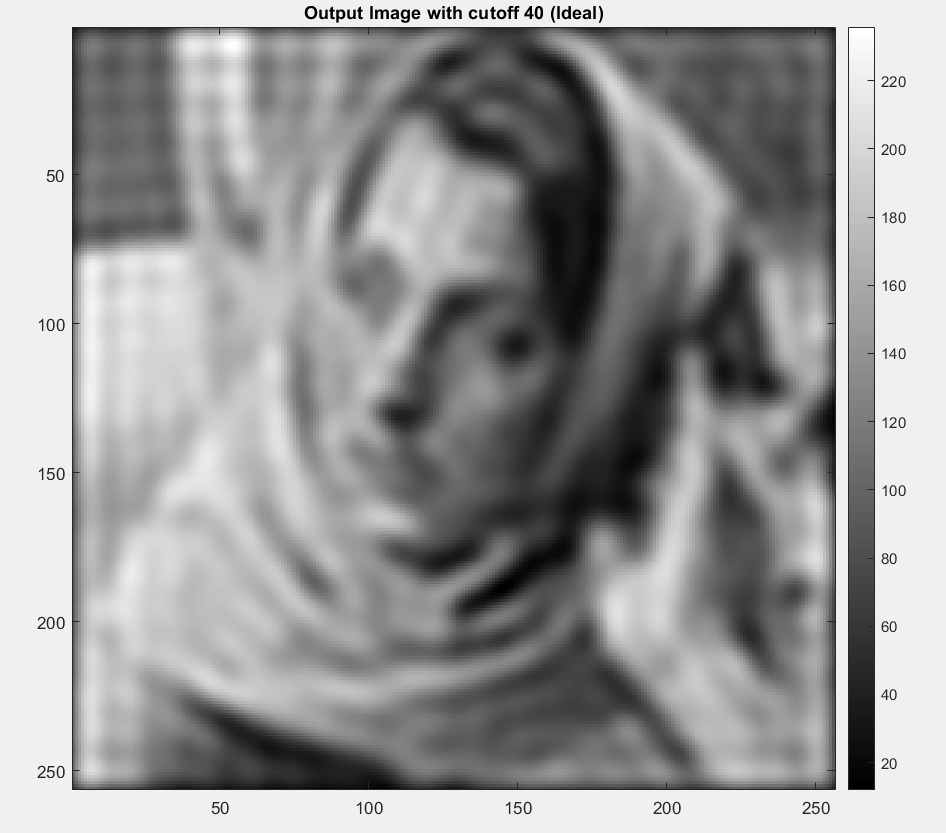
\includegraphics[width=\linewidth]{Screenshot (265).png}
    \caption{Output Image after applying ideal LPF}
  \end{subfigure}
  \begin{subfigure}[b]{0.37\linewidth}
    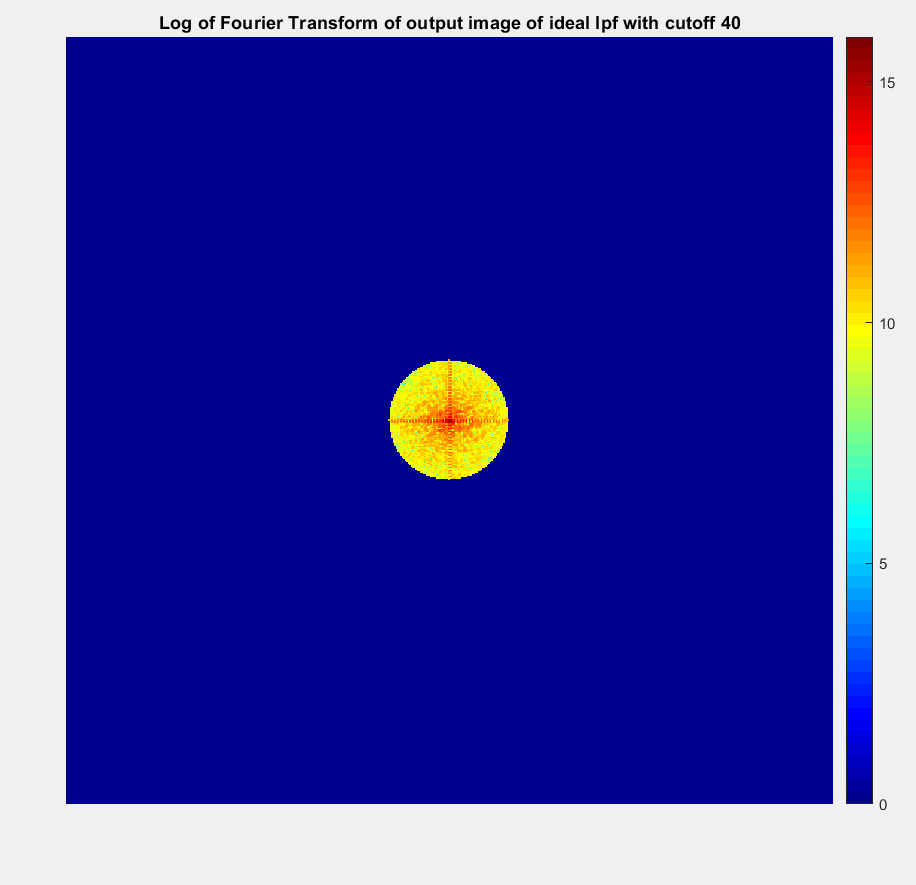
\includegraphics[width=\linewidth]{Screenshot (266).png}
    \caption{Fourier Transform of the Image}
  \end{subfigure}
  \caption{}
  \label{fig:3}
\end{figure}


\subsection{Cutoff frequency $|D|=80$}
The frequency response corresponding the filter is shown below.
\begin{figure}[h!]
  \centering
    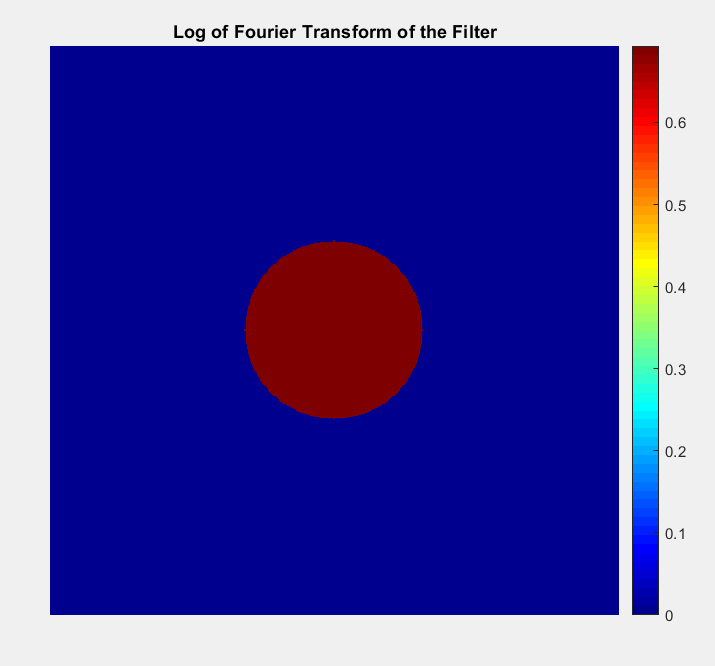
\includegraphics[scale=0.4]{Screenshot (277).png}
    \caption{Frequency response of an ideal LPF with cutoff frequency $|\omega|=80$}
  \label{fig:4}
\end{figure}

\clearpage

Image and the corresponding Fourier Transform are shown in fig. given below.
\begin{figure}[H]
  \centering
  \begin{subfigure}[b]{0.45\linewidth}
    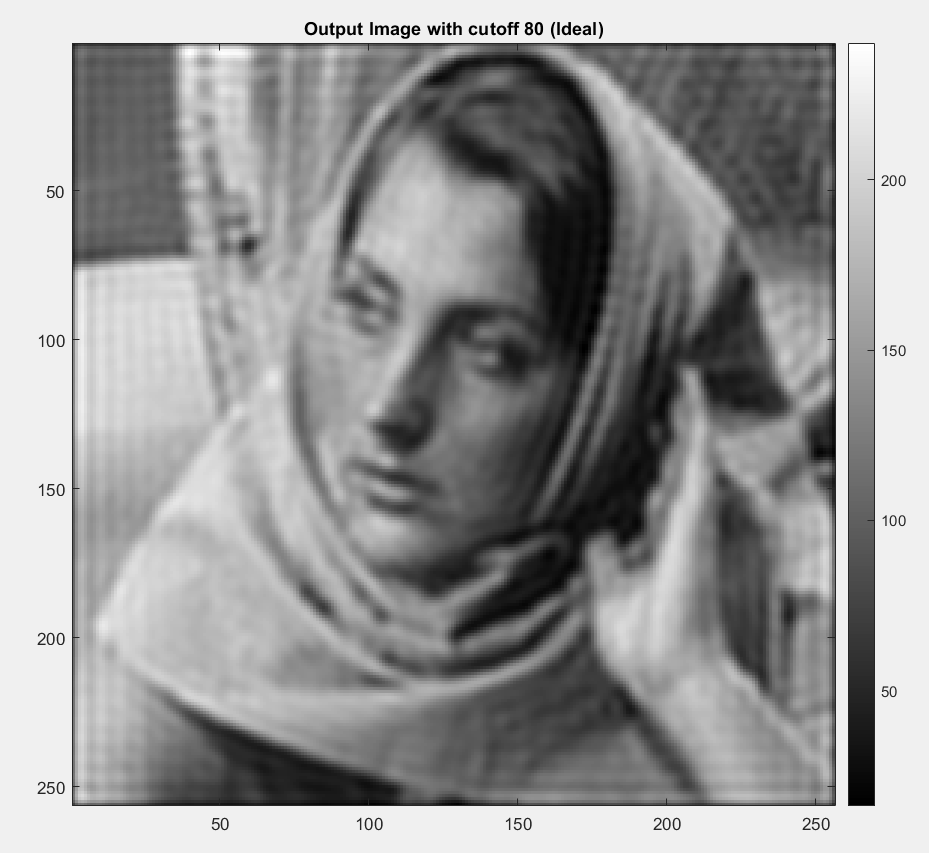
\includegraphics[width=\linewidth]{Screenshot (267).png}
    \caption{Output Image after applying ideal LPF}
  \end{subfigure}
  \begin{subfigure}[b]{0.45\linewidth}
    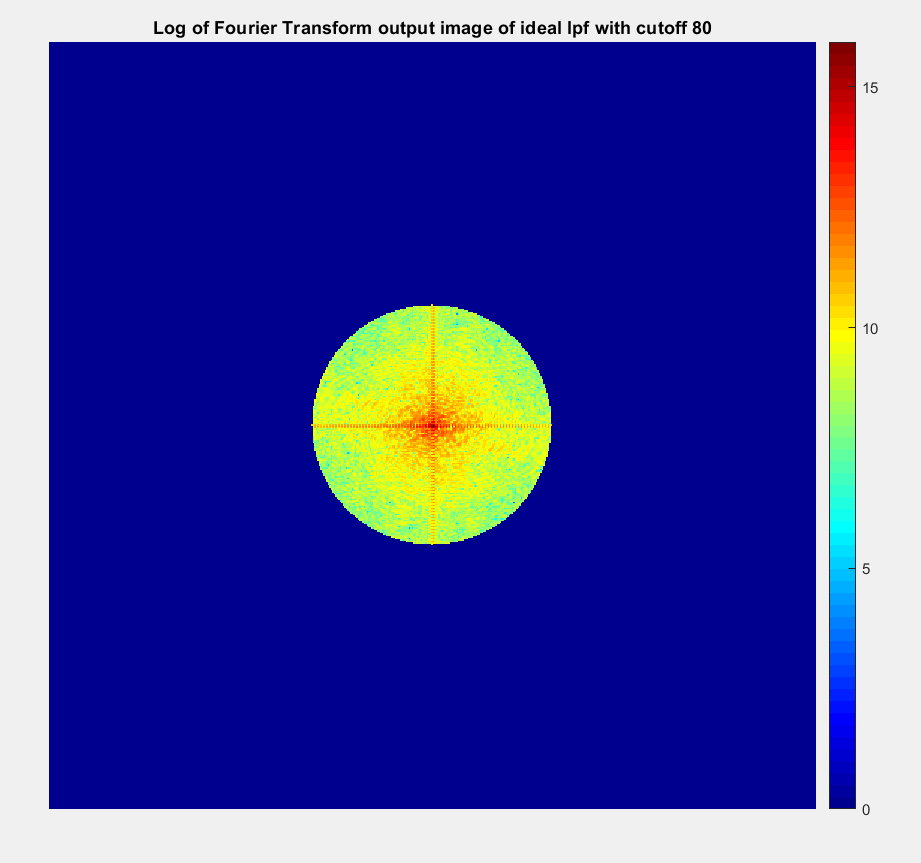
\includegraphics[width=\linewidth]{Screenshot (268).png}
    \caption{Fourier Transform of the Image}
  \end{subfigure}
  \caption{}
  \label{fig:5}
\end{figure}

\section{Gaussian low pass filter}
\subsection{Standard Deviation $\sigma=40$}
The frequency response corresponding the filter is shown below.
\begin{figure}[h!]
  \centering
    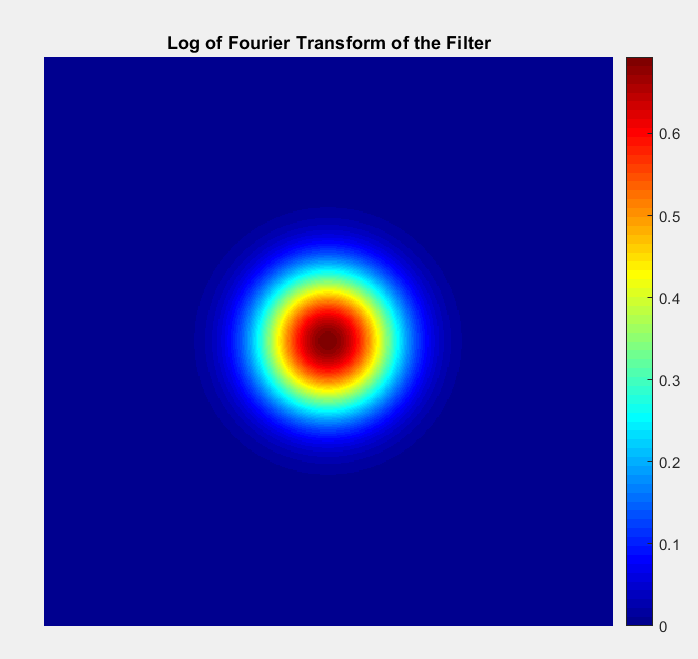
\includegraphics[scale=0.4]{Screenshot (278).png}
    \caption{Frequency response of an Gaussian LPF with standard deviation $|\sigma|=40$}
  \label{fig:6}
\end{figure}

\clearpage

Image and the corresponding Fourier Transform are shown in fig. given below.
\begin{figure}[H]
  \centering
  \begin{subfigure}[b]{0.45\linewidth}
    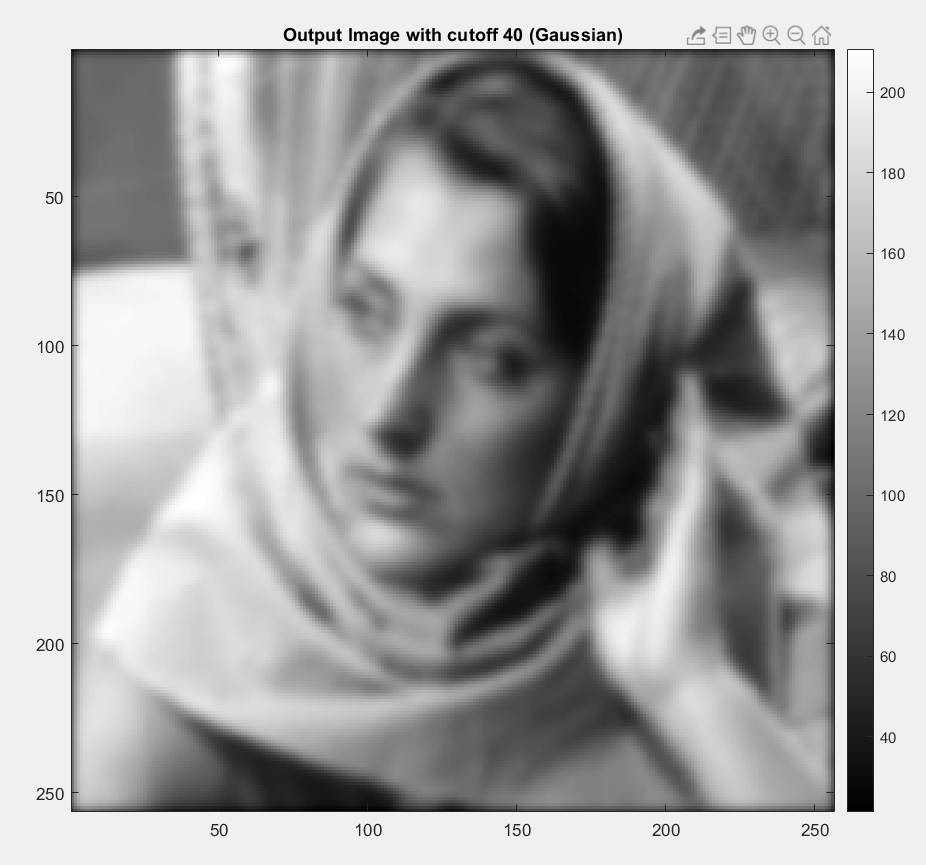
\includegraphics[width=\linewidth]{Screenshot (269).png}
    \caption{Output Image after applying Gaussian LPF}
  \end{subfigure}
  \begin{subfigure}[b]{0.45\linewidth}
    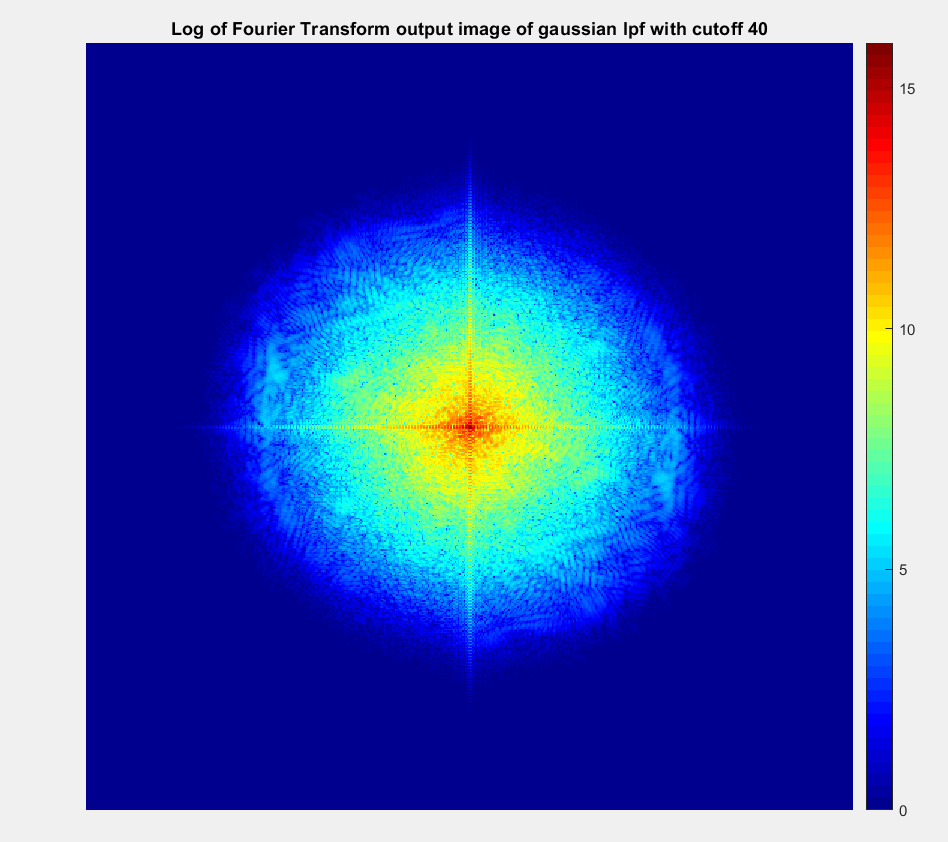
\includegraphics[width=\linewidth]{Screenshot (270).png}
    \caption{Fourier Transform of the Image}
  \end{subfigure}
  \caption{}
  \label{fig:7}
\end{figure}

\subsection{Standard Deviation $\sigma=80$}
The frequency response corresponding the filter is shown below.
\begin{figure}[h!]
  \centering
    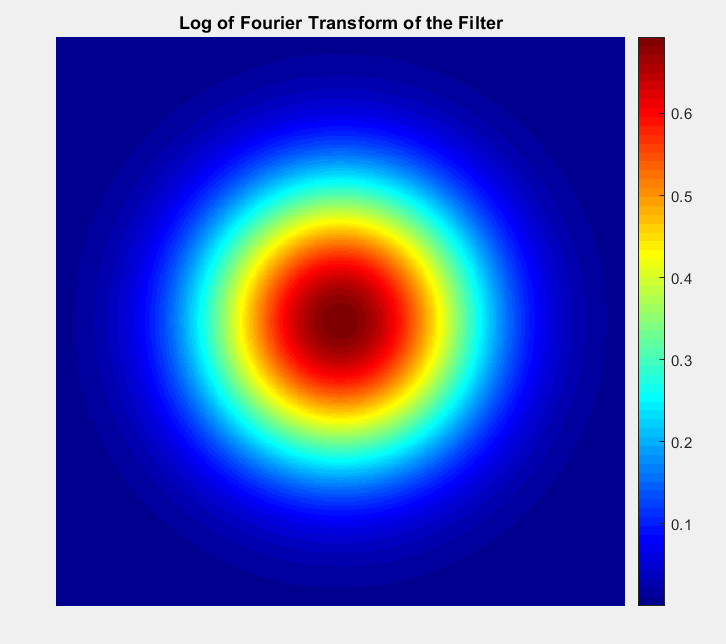
\includegraphics[scale=0.4]{Screenshot (279).png}
    \caption{Frequency response of an Gaussian LPF with standard deviation $|\sigma|=80$}
  \label{fig:8}
\end{figure}

\clearpage

Image and the corresponding Fourier Transform are shown in fig. given below.
\begin{figure}[H]
  \centering
  \begin{subfigure}[b]{0.45\linewidth}
    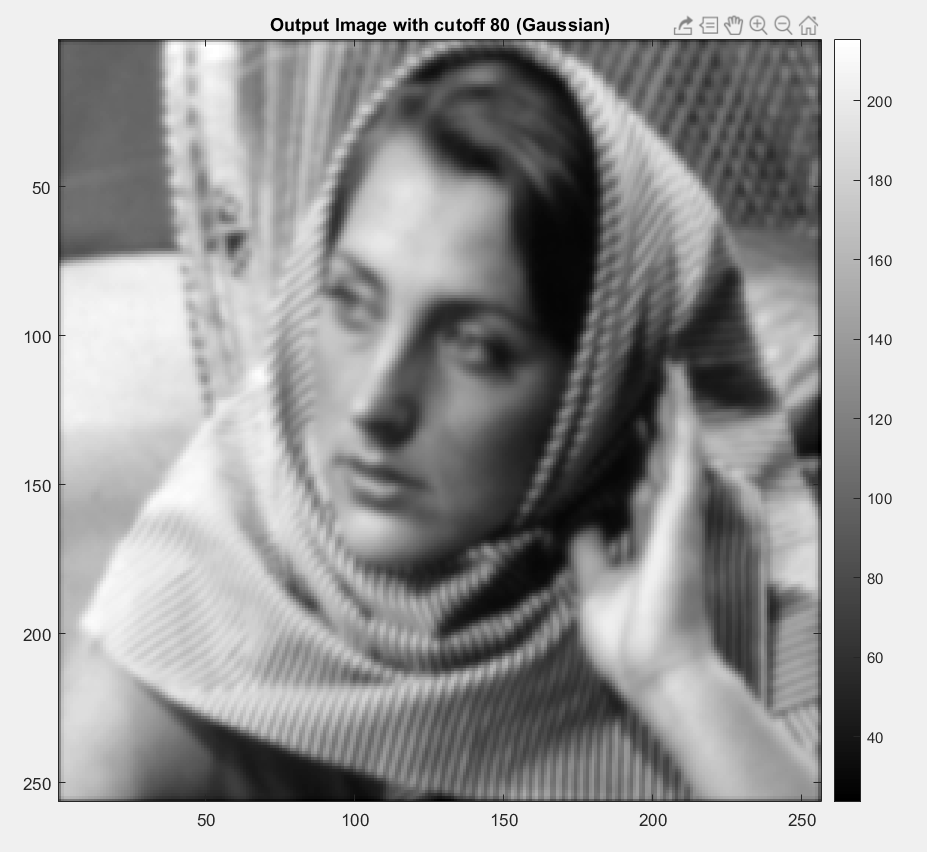
\includegraphics[width=\linewidth]{Screenshot (271).png}
    \caption{Output Image after applying Gaussian LPF}
  \end{subfigure}
  \begin{subfigure}[b]{0.45\linewidth}
    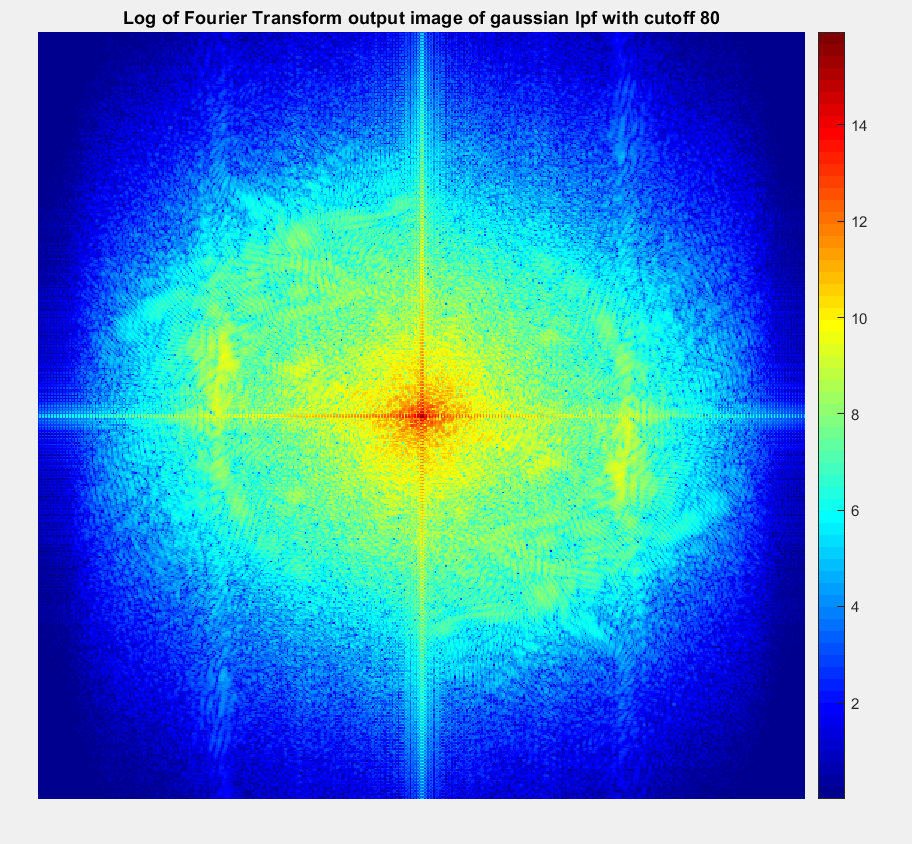
\includegraphics[width=\linewidth]{Screenshot (272).png}
    \caption{Fourier Transform of the Image}
  \end{subfigure}
  \caption{}
  \label{fig:9}
\end{figure}

\section{Explanation}
We can see a stark difference in the output image which was expected also. The idea LPF corresponds to jinc function in the spatial domain which gives rippling or ringing effect in the image. As the size of the LPF is increased the ringing effect also decreases. The Fourier Transform of a Gaussian Filter gives a Gaussian kernel in the spatial domain also which is essentially Gaussian smoothening of the image.

\section{Code Usage}
The code is divided into three parts.
\begin{itemize}
    \item Part 1 is just extracts the image from the folder and displays it and its Fourier Transform.
    \item Part 2 corresponds to an LTI system which is an ideal LPF with cutoff frequencies, f$\in\{40, 80\}$. 
    \item Part 3 corresponds to an LTI system which is a Gaussian LPF with standard deviation, $\sigma\in\{40, 80\}$. 
\end{itemize}
\end{document}
